\documentclass[11pt,aspectratio=169]{beamer}

\usetheme{metropolis}
\usecolortheme{default}
\metroset{numbering=fraction, progressbar=frametitle, sectionpage=none}

\setbeamertemplate{navigation symbols}{}
\setbeamercolor{frametitle}{bg=mDarkTeal, fg=white}
\setbeamercolor{progress bar}{fg=mDarkTeal, bg=mDarkTeal!20}
\definecolor{mDarkTeal}{HTML}{23373B}
\definecolor{mAccent}{HTML}{EB811B}

\usepackage{amsmath,amssymb}
\usepackage{graphicx}
\usepackage{booktabs}
\usepackage{appendixnumberbeamer}
\usepackage{tikz}
\usepackage{wasysym}

\title{Math Bootcamp}
\subtitle{Day 1 --- Foundations (Sections 1.1--1.7)}
\author{Math Camp 2026}
\date{}

\newcommand{\QFrame}[1]{%
  \begin{frame}{#1 \quad {\small\textcolor{mAccent}{Together}}}}

\begin{document}

\begin{frame}
  \titlepage
\end{frame}

\section{1.1 --- Notation and Number Systems}

\begin{frame}{1.1 Number systems --- names and definitions}
  \small
  \begin{tabular}{@{}clp{0.48\textwidth}@{}}
    \toprule
    \textbf{Symbol} & \textbf{English name} & \textbf{What it is} \\
    \midrule
    $\mathbb{N}$ & natural numbers & Non-negative integers for \textbf{counting} \\
    $\mathbb{Z}$ & integers & $\ldots,-2,-1,0,1,2,\ldots$ \\
    $\mathbb{Q}$ & rational numbers & Fractions $p/q$ ($q\ne0$) \\
    $\mathbb{R}$ & real numbers & All points on the number line \\
    $\mathbb{R}^n$ & $n$-dimensional real space & Lists / vectors of length $n$ \\
    \bottomrule
  \end{tabular}

  \medskip
  \begin{center}
  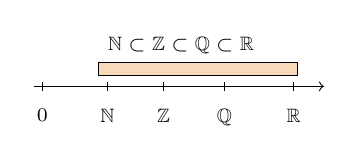
\begin{tikzpicture}[scale=0.55, every node/.style={font=\scriptsize}]
    \draw[->] (-0.2,0) -- (6.5,0);
    \foreach \x/\lab in {0/0,1.5/$\mathbb{N}$,2.8/$\mathbb{Z}$,4.2/$\mathbb{Q}$,5.8/$\mathbb{R}$}
      \draw (\x,0.1) -- (\x,-0.1) node[below=3pt] {\lab};
    \draw[fill=mAccent!30] (1.3,0.25) rectangle (5.9,0.55);
    \node at (3.2,0.95) {$\mathbb{N}\subset\mathbb{Z}\subset\mathbb{Q}\subset\mathbb{R}$};
  \end{tikzpicture}
  \end{center}
\end{frame}

\begin{frame}{1.1 Symbols and vectors --- names and definitions}
  \textbf{Common symbols}
  \small
  \begin{tabular}{@{}cl@{\quad}cl@{}}
    $\in$ & ``is an element of'' &
    $\forall$ & ``for all'' \\
    $\exists$ & ``there exists'' &
    $\Rightarrow$ & ``implies'' \\
    & &
    $\Leftrightarrow$ & ``if and only if'' (iff) \\
  \end{tabular}

  \medskip
  \normalsize
  \textbf{Scalar vs.\ vector}
  \small
  \begin{itemize}
    \item \textbf{Scalar:} one number, e.g.\ income $w\in\mathbb{R}$
    \item \textbf{Vector:} a list of numbers
      $\mathbf{x}=(x_1,\ldots,x_n)\in\mathbb{R}^n$
    \item \textbf{Dot product:} $\mathbf{p}\cdot\mathbf{x}=\sum_{i=1}^n p_i x_i$
  \end{itemize}
\end{frame}

\QFrame{1.1 --- Which set?}
  \small
  \textbf{Smallest set that fits?}

  \medskip
  \onslide<2->{\textbf{1.} The number of girlfriends / boyfriends you can have\par}
  \onslide<3->{\textcolor{mAccent}{$\rightarrow\;\mathbb{N}$}\hfill
    {\scriptsize counting: $0,1,2,\ldots$}\par\medskip}

  \onslide<4->{\textbf{2.} Money you spend at a vending machine (e.g.\ HK\$8.50)\par}
  \onslide<5->{\textcolor{mAccent}{$\rightarrow\;\mathbb{Q}$}\hfill
    {\scriptsize e.g.\ $8.50=17/2$ dollars}\par\medskip}

  \onslide<6->{\textbf{3.} Order as a vector: (HK\$ spent on drink, \# snacks) = $(8.50,\,2)$\par}
  \onslide<7->{\textcolor{mAccent}{$\rightarrow\;(8.50,\,2)\in\mathbb{Q}\times\mathbb{N}$}\par}
\end{frame}

\section{1.2 --- Logic and Mathematical Statements}

\begin{frame}{1.2 Logic --- names and definitions}
  \footnotesize
  \begin{tabular}{@{}llp{0.52\textwidth}@{}}
    \toprule
    \textbf{English} & \textbf{Symbol} & \textbf{Meaning} \\
    \midrule
    $P$ \textbf{only if} $Q$ & $P\Rightarrow Q$ &
      $Q$ is \textbf{necessary} for $P$ (without $Q$, no $P$) \\[4pt]
    $P$ \textbf{if} $Q$ & $Q\Rightarrow P$ &
      $Q$ is \textbf{sufficient} for $P$ ($Q$ alone is enough) \\[4pt]
    $P$ \textbf{if and only if} $Q$ & $P\Leftrightarrow Q$ &
      $Q$ is necessary \textbf{and} sufficient \\[4pt]
    \textbf{Contrapositive} & $\neg Q\Rightarrow\neg P$ &
      same truth as $P\Rightarrow Q$:\\
    & & if $Q$ fails, $P$ must fail \\
    \bottomrule
  \end{tabular}
\end{frame}

\QFrame{1.1 --- IKEA run}
  \footnotesize
  \textbf{First week in HK:} you go to IKEA and spot three plush toys.

  \medskip
  \begin{columns}[T,onlytextwidth]
    \column{0.32\textwidth}
    \centering
    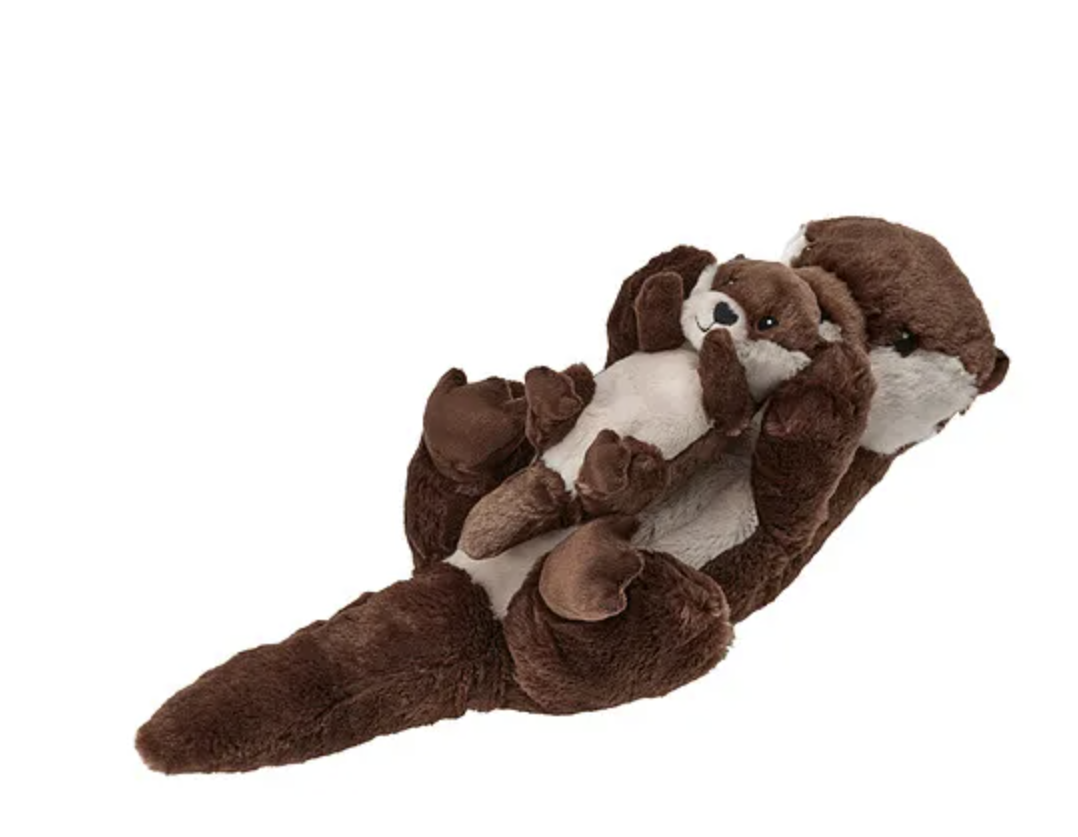
\includegraphics[width=\linewidth]{figures/otter.png}\\[2pt]
    Otter \quad HK\$179.9

    \column{0.32\textwidth}
    \centering
    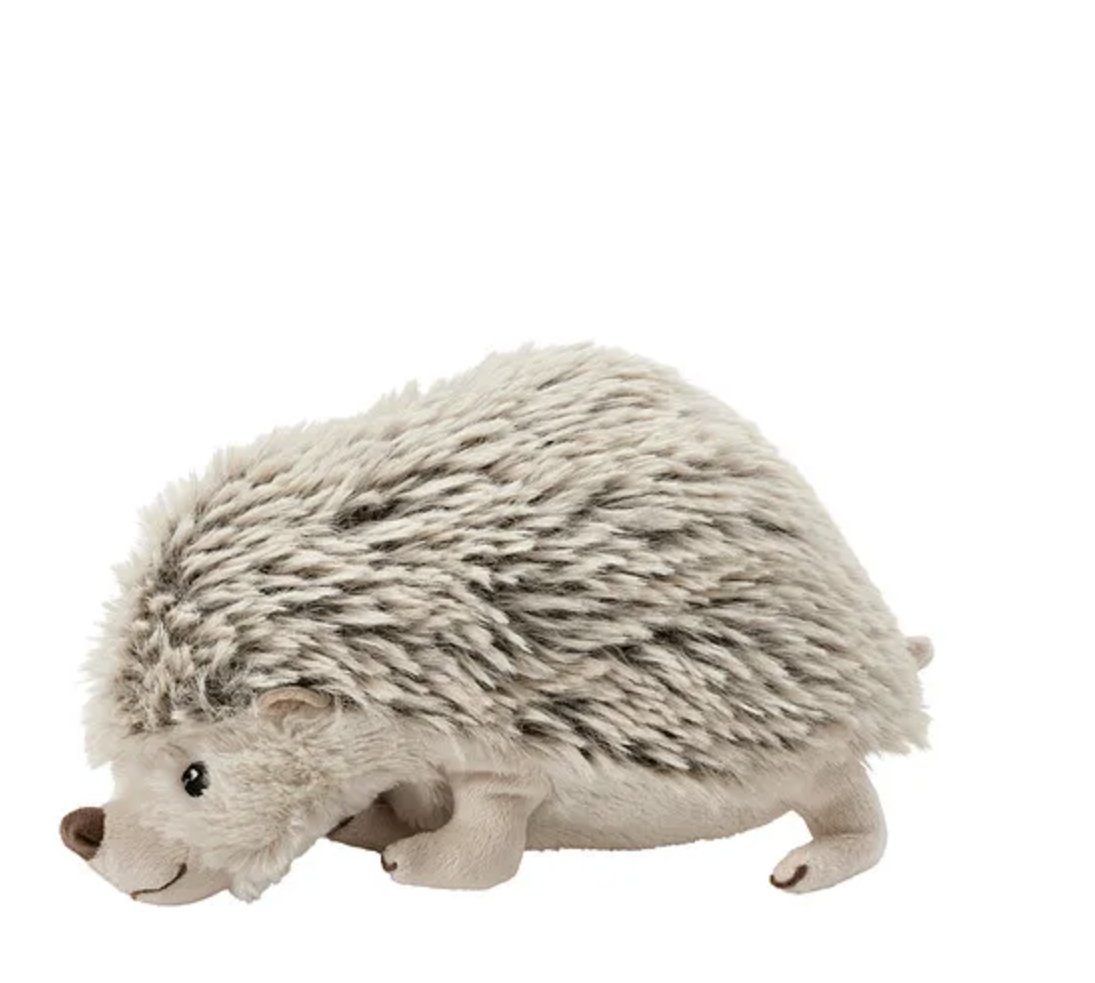
\includegraphics[width=\linewidth]{figures/hedgehog.png}\\[2pt]
    Hedgehog \quad HK\$79.9

    \column{0.32\textwidth}
    \centering
    
\includegraphics[width=\linewidth]{figures/shark.jpg}\\[2pt]
    BLÅHAJ \quad HK\$179.9
  \end{columns}

  \medskip
  You have \textbf{HK\$500} pocket money ($B=500$).

  \medskip
  Basket $\mathbf{x}\in\mathbb{N}^3$: \# otters, \# hedgehogs, \# sharks.
  E.g.\ $(1,\,1,\,0)$ = one otter, one hedgehog, no shark.
  Price vector $\mathbf{p}=(179.9,\,79.9,\,179.9)\in\mathbb{Q}^3$.
  Budget set:
  $\mathcal{B}=\{\mathbf{x}\in\mathbb{N}^3:\mathbf{p}\cdot\mathbf{x}\le 500\}$.
\end{frame}

\QFrame{1.2 --- Plush symbols practice}
  \scriptsize
  $\mathbf{p}=(179.9,\,79.9,\,179.9)$,\ $\mathcal{B}=\{\mathbf{x}\in\mathbb{N}^3:\mathbf{p}\cdot\mathbf{x}\le 500\}$.
  \textbf{True or false?}

  \vspace{2pt}
  \onslide<2->{\textbf{1.} [$\in$]\ $(0,0,3)\in\mathcal{B}$}\;
  \onslide<3->{\textcolor{mAccent}{\textbf{False}} {\tiny ($539.7>500$)}}\par
  \onslide<4->{\textbf{2.} [$\subset$]\ $\mathbb{N}^3\subset\mathcal{B}$}\;
  \onslide<5->{\textcolor{mAccent}{\textbf{False}} {\tiny (e.g.\ $(3,0,0)\notin\mathcal{B}$)}}\par
  \onslide<6->{\textbf{3.} [$\forall$]\ $\forall\,\mathbf{x}\in\mathcal{B},\;\mathbf{x}\ne(0,1,0)$}\;
  \onslide<7->{\textcolor{mAccent}{\textbf{False}} {\tiny ($(0,1,0)\in\mathcal{B}$)}}\par
  \onslide<8->{\textbf{4.} [$\exists$]\ $\exists\,\mathbf{x}\in\mathcal{B},\;\mathbf{x}=(3,0,0)$}\;
  \onslide<9->{\textcolor{mAccent}{\textbf{False}} {\tiny ($539.7>500$)}}\par
  \onslide<10->{\textbf{5.} [$\Rightarrow$]\ $(1,1,1)\in\mathcal{B}$ \textbf{only if}
    $\mathbf{p}\cdot(1,1,1)\le 500$}\;
  \onslide<11->{\textcolor{mAccent}{\textbf{True}} {\tiny ($439.7\le 500$)}}\par
  \onslide<12->{\hspace{1.5em}{\tiny also True: $(1,1,1)\in\mathcal{B}$ \textbf{if}
    $\mathbf{p}\cdot(1,1,1)\le 500$}}\par
  \onslide<13->{\textbf{6.} [$\Rightarrow$]\ $(0,0,3)\in\mathcal{B}$ \textbf{if}
    $(1,1,1)\in\mathcal{B}$}\;
  \onslide<14->{\textcolor{mAccent}{\textbf{False}} {\tiny ($(1,1,1)\in\mathcal{B}$ but $539.7>500$)}}\par
  \onslide<15->{\textbf{7.} [contrapositive]\ If
    $\mathbf{p}\cdot(1,1,1)+\mathbf{p}\cdot(0,1,0)>500$, then
    $(1,1,1)\notin\mathcal{B}$ \textbf{or} $(0,1,0)\notin\mathcal{B}$}\;
  \onslide<16->{\textcolor{mAccent}{\textbf{False}} {\tiny ($519.6>500$, yet each basket alone is in $\mathcal{B}$)}}\par
  \onslide<17->{\hspace{1.5em}{\tiny each affordable $\not\Rightarrow$ jointly affordable}}\par
\end{frame}

\section{1.3 --- Sets and Set Operations}

\begin{frame}{1.3 Sets and operations --- names and definitions}
  \scriptsize
  \begin{tabular}{@{}clp{0.38\textwidth}@{}}
    \toprule
    \textbf{Symbol} & \textbf{Name} & \textbf{Meaning} \\
    \midrule
    $\in$, $\notin$ & element / not in & $x$ belongs (or not) to $A$ \\
    $\subset$, $=$ & subset, equality & $A\subset B$; $A=B$ iff mutual $\subset$ \\
    $\emptyset$, $\{\,\}$, $\{x\in S:\ldots\}$ & sets & empty, roster, set-builder \\
    $A\cup B$, $A\cap B$ & union, intersection & in $A$ or $B$; in both \\
    $A^c$, $A\setminus B$ & complement, difference & not in $A$; in $A$ not $B$ \\
    $A\times B$ & Cartesian product & pairs $(a,b)$, $a\in A$, $b\in B$ \\
    \bottomrule
  \end{tabular}

  \medskip
  \textbf{In economics:}\quad
  budget set $\mathcal{B}\subset\mathbb{N}^3$;\;
  $(8.50,\,2)\in\mathbb{Q}\times\mathbb{N}$.
\end{frame}

\QFrame{1.3 --- Set operations (IKEA)}
  \scriptsize
  $\mathcal{B}=\{\mathbf{x}\in\mathbb{N}^3:\mathbf{p}\cdot\mathbf{x}\le 500\}$,\quad
  $\mathcal{H}=\{\mathbf{x}\in\mathbb{N}^3:\text{middle entry}\ge 1\}$ (at least one hedgehog).

  \vspace{2pt}
  \textbf{Describe the set.}

  \vspace{2pt}
  \onslide<2->{\textbf{1.} $\mathcal{B}\cap\mathcal{H}$}\;
  \onslide<3->{\textcolor{mAccent}{affordable baskets with $\ge 1$ hedgehog}
    {\tiny (e.g.\ $(0,1,0)$)}}\par
  \onslide<4->{\textbf{2.} $\mathcal{B}\cup\mathcal{H}$}\;
  \onslide<5->{\textcolor{mAccent}{affordable baskets \textbf{or} baskets with $\ge 1$ hedgehog}}\par
  \onslide<6->{\textbf{3.} $\mathcal{B}\setminus\mathcal{H}$}\;
  \onslide<7->{\textcolor{mAccent}{affordable baskets with \textbf{no} hedgehog}
    {\tiny (e.g.\ $(1,0,0)$)}}\par
  \onslide<8->{\textbf{4.} $(179.9,\,79.9)\in\mathbb{Q}\times\mathbb{Q}$ but
    $(179.9,\,79.9)\notin\mathcal{B}$}\;
  \onslide<9->{\textcolor{mAccent}{True}\;
    {\tiny Cartesian product $\ne$ budget set --- pairs $\ne$ baskets}}\par
  \onslide<10->{\textbf{5.} $(1,0,0)\subset\mathcal{B}$}\;
  \onslide<11->{\textcolor{mAccent}{\textbf{False}}\;
    {\tiny $(1,0,0)$ is a basket: use $(1,0,0)\in\mathcal{B}$ (True);
    but $\{(1,0,0)\}\subset\mathcal{B}$ is True}}\par
\end{frame}

\section{1.4 --- Functions}

\begin{frame}{1.4 Functions --- names and definitions}
  \scriptsize
  \begin{tabular}{@{}clp{0.40\textwidth}@{}}
    \toprule
    \textbf{Term} & \textbf{Notation} & \textbf{Meaning} \\
    \midrule
    Function & $f\colon A\to B$ & each $x\in A$ maps to \textbf{exactly one} $f(x)\in B$ \\
    Domain & $A$ & allowed inputs \\
    Codomain & $B$ & target set --- every output must lie in $B$ \\
    Range & $f(A)$ & outputs hit: $\{f(x):x\in A\}\subseteq B$ \\
    Injective (one-to-one) &  & $f(x_1)=f(x_2)\Rightarrow x_1=x_2$ \\
    Surjective (onto) &  & every $y\in B$ equals some $f(x)$ \\
    Operations & $(f\pm g)(x)$, $(cf)(x)$, $(fg)(x)$ &
      $(f\pm g)(x)=f(x)\pm g(x)$;\ $(cf)(x)=c\,f(x)$;\ $(fg)(x)=f(x)g(x)$ \\
    Composition & $(f\circ g)(x)$ & apply $g$ first: $(f\circ g)(x)=f(g(x))$ \\
    \bottomrule
  \end{tabular}
\end{frame}

\QFrame{1.4 --- Ages}
  \small
  Define $f\colon D\to C$ by: $f(x)$ = your girlfriend / boyfriend's age
  when \textbf{your age} is $x$.

  \vspace{4pt}
  \onslide<2->{\textbf{1.} Domain $D$?}\;
  \onslide<3->{\textcolor{mAccent}{$\{22,23,\ldots,30\}$}\hfill
    {\scriptsize typical ages in a master's program}}\par
  \onslide<4->{\textbf{2.} Codomain $C$?}\;
  \onslide<5->{\textcolor{mAccent}{$\{18,19,\ldots,120\}$}\hfill
    {\scriptsize plausible partner ages}}\par
  \onslide<6->{\textbf{3.} Is $80\in f(D)$?}\;
  \onslide<7->{\textcolor{mAccent}{\textbf{Probably not}}\hfill
    {\scriptsize ($80\in C$, but $f(D)\subseteq\{17,\ldots,35\}$)}}\par
  \onslide<8->{\textbf{4.} Range $f(D)$?}\;
  \onslide<9->{\textcolor{mAccent}{your age $\pm 5$ on $D$}\hfill
    {\scriptsize $\{17,18,\ldots,35\}$}}\par
  \onslide<10->{\textbf{5.} Is $f$ surjective (onto $C$)?}\;
  \onslide<11->{\textcolor{mAccent}{\textbf{No}}\hfill
    {\scriptsize ($f(D)\ne C$; e.g.\ $120\in C$ but $120\notin f(D)$)}}\par
  \onslide<12->{\textbf{6.} Is $f$ injective (one-to-one)?}\;
  \onslide<13->{\textcolor{mAccent}{\textbf{Probably not}}\hfill
    {\scriptsize (e.g.\ $f(22)=f(30)=22$)}}\par
  \onslide<14->{\textbf{7.} If $f(25)=\{22,\,80\}$, is $f$ a function?}\;
  \onslide<15->{\textcolor{mAccent}{\textbf{No --- a correspondence}}\hfill
    {\scriptsize (a function gives \textbf{exactly one} output per input;
    it's immoral to have a correspondence\ \smiley)}}\par
\end{frame}

\section{1.5 --- Supremum and Infimum}

\QFrame{1.5 --- Reservation price (example first)}
  \small
  BLÅHAJ sticker price: \textbf{HK\$179.9}.
  You buy \textbf{only on sale}: when $p<179.9$.

  \medskip
  Prices where you still buy:
  $P=\{p\in\mathbb{R}_+:p<179.9\}$.

  \vspace{4pt}
  \onslide<2->{\textbf{Highest sale price you would accept?}}\;
  \onslide<3->{\textcolor{mAccent}{\textbf{No maximum in $P$}}\hfill
    {\scriptsize ($179.89$ works; so does $179.899$; \ldots)}}\par
  \onslide<4->{\textbf{Reservation price (WTP)?}}\;
  \onslide<5->{\textcolor{mAccent}{$\sup P=179.9$}\hfill
    {\scriptsize least upper bound --- the choke price)}}\par
  \onslide<6->{\textbf{Is $179.9\in P$?}}\;
  \onslide<7->{\textcolor{mAccent}{\textbf{No}}\hfill
    {\scriptsize at sticker price you walk away $\Rightarrow$ no $\max P$)}}\par
\end{frame}

\begin{frame}{1.5 Supremum and infimum --- names and definitions}
  \scriptsize
  \begin{tabular}{@{}clp{0.40\textwidth}@{}}
    \toprule
    \textbf{Term} & \textbf{Notation} & \textbf{Meaning} \\
    \midrule
    Maximum & $\max S$ & largest element \textbf{in} $S$ \\
    Minimum & $\min S$ & smallest element \textbf{in} $S$ \\
    Supremum & $\sup S$ & \textbf{least upper bound} of $S$ \\
    Infimum & $\inf S$ & \textbf{greatest lower bound} of $S$ \\
    \bottomrule
  \end{tabular}

  \medskip
  \textbf{Example (least upper bound):}\quad
  $S=[0,1)$.\ Upper bounds include $1,2,3,\ldots$;
  $\sup S=1$ --- the \textbf{smallest} upper bound ($1\notin S$).

  \medskip
  \textbf{Relations:}\quad
  if $\max S$ exists, $\max S=\sup S$;\ if $\min S$ exists, $\min S=\inf S$.

  \smallskip
  \hspace{2.1em}Always: $\inf S\le x\le\sup S$ for all $x\in S$.
\end{frame}

\section{1.6 --- Algebra Revision}

\begin{frame}{1.6 Taylor, logs, and exponentials}
  \scriptsize
  \textbf{Taylor expansion} (around $a$):
  \[
    f(a+h)=\sum_{k=0}^{\infty}\frac{f^{(k)}(a)}{k!}\,h^k
    =f(a)+f'(a)h+\frac{f''(a)}{2!}h^2+\frac{f^{(3)}(a)}{3!}h^3+\cdots
  \]

  \medskip
  \begin{tabular}{@{}ll@{\quad}ll@{}}
    \textbf{Logs} & & \textbf{Exponentials} & \\
    $\ln(ab)=\ln a+\ln b$ & & $e^{a+b}=e^a e^b$ & \\
    $\ln(x^\alpha)=\alpha\ln x$ & & $e^{\alpha x}=(e^x)^\alpha$ & \\
    $\ln(1+x)=x-\dfrac{x^2}{2}+\dfrac{x^3}{3}-\cdots$ & & $e^x=1+x+\dfrac{x^2}{2!}+\cdots$ & \\
  \end{tabular}

  \medskip
  \textbf{Quick check:}\quad
  $\ln(x_1^\alpha x_2^\beta)=\alpha\ln x_1+\beta\ln x_2$;\quad
  if $u=x_1^\alpha x_2^{1-\alpha}$, then
  $\ln u=\alpha\ln x_1+(1-\alpha)\ln x_2$.
\end{frame}

\begin{frame}{1.6 Why logs?}
  \small
  \begin{itemize}
    \item \textbf{Taylor:}\quad
      $f(a+h)\approx f(a)+f'(a)h$.
    \item \textbf{Apply to logs:}\quad
      $\ln(1+x)\approx x$ for small $x$.
    \item \textbf{Percentage changes:}\quad
      $\ln(x+\Delta x)-\ln x=\ln\!\bigl(1+\tfrac{\Delta x}{x}\bigr)\approx \tfrac{\Delta x}{x}$,
      so $\Delta\ln x$ tracks \textbf{\% change} in $x$.
    \item \textbf{Example:}\quad
      $\tfrac{\Delta x}{x}=5\%\Rightarrow \Delta\ln x\approx 0.05$.
    \item \textbf{Log--log regression:}\quad
      $\ln y=\alpha+\beta\ln x$.
    \item 1\% $\uparrow$ in $x$ $\Rightarrow$ $\beta$\% change in $y$.
    \item \textbf{Elasticity:}\quad
      $\varepsilon_{y,x}=\dfrac{\partial y}{\partial x}\dfrac{x}{y}
      =\dfrac{\Delta y/y}{\Delta x/x}
      =\dfrac{\partial\ln y}{\partial\ln x}$;\quad
      in $\ln y=\alpha+\beta\ln x$, $\varepsilon_{y,x}=\beta$.
  \end{itemize}
\end{frame}

\begin{frame}{1.6 Cobb--Douglas --- definition}
  \small
  \textbf{Utility / production:}
  \[
    U(x_1,x_2)=x_1^{\alpha}x_2^{1-\alpha},\qquad
    Y(K,L)=A K^{\alpha}L^{1-\alpha},\quad \alpha\in(0,1).
  \]

  \medskip
  \textbf{In logs (linear):}\quad
  $\ln U=\alpha\ln x_1+(1-\alpha)\ln x_2$;\quad
  $\ln Y=\ln A+\alpha\ln K+(1-\alpha)\ln L$.

  \medskip
  \textbf{Constant elasticity:}
  $\varepsilon_{U,x_1}=\dfrac{\partial\ln U}{\partial\ln x_1}=\alpha$,\quad
  $\varepsilon_{U,x_2}=1-\alpha$;\quad
  $\varepsilon_{Y,K}=\alpha$,\ $\varepsilon_{Y,L}=1-\alpha$.
  {\scriptsize Same numbers at every $(x_1,x_2)$ or $(K,L)$.}
\end{frame}

\begin{frame}{1.6 Why Cobb--Douglas? --- first-order approximation}
  \small
  \textbf{Any smooth utility $u(x_1,x_2)>0$:}\quad
  define $f(\ln x_1,\ln x_2)=\ln u(x_1,x_2)$.

  \medskip
  \textbf{First-order Taylor} around $(\ln\bar x_1,\ln\bar x_2)$:
  \[
    \ln u(x_1,x_2)
    \approx
    f(\ln\bar x_1,\ln\bar x_2)
    +\frac{\partial f}{\partial\ln x_1}\Big|_{\bar{\mathbf{x}}}(\ln x_1-\ln\bar x_1)
    +\frac{\partial f}{\partial\ln x_2}\Big|_{\bar{\mathbf{x}}}(\ln x_2-\ln\bar x_2).
  \]

  \medskip
  Let $\alpha_i=\dfrac{\partial\ln u}{\partial\ln x_i}\Big|_{\bar{\mathbf{x}}}$
  and absorb constants into $c$:
  \[
    \ln u(x_1,x_2)\approx c+\alpha_1\ln x_1+\alpha_2\ln x_2
    \quad\Leftrightarrow\quad
    u(x_1,x_2)\approx e^c\,x_1^{\alpha_1}x_2^{\alpha_2}.
  \]

  \medskip
  {\scriptsize Near $\bar{\mathbf{x}}$ only; Cobb--Douglas is exact when $\ln u$ is globally affine in logs.}
\end{frame}

\begin{frame}{1.6 Cobb--Douglas --- homogeneity and CRS}
  \scriptsize
  \textbf{Homogeneous of degree $k$:}\quad
  $f(t\mathbf{x})=t^k f(\mathbf{x})$ for $t>0$.

  \medskip
  \textbf{Utility}\ $U=x_1^{\alpha}x_2^{1-\alpha}$:\quad
  $U(tx_1,tx_2)=t^{\alpha}t^{1-\alpha}U(\mathbf{x})=t\,U(\mathbf{x})$
  $\Rightarrow$ degree~$1$.

  \medskip
  \textbf{Production}\ $Y=A K^{\alpha}L^{1-\alpha}$:\quad
  $Y(tK,tL)=t^{\alpha}t^{1-\alpha}Y(K,L)=t\,Y(K,L)$.

  \medskip
  \textbf{CRS (constant returns to scale):}\quad
  double all inputs $\Rightarrow$ double output (homogeneous of degree~$1$).
\end{frame}

\begin{frame}{1.6 Cobb--Douglas --- constant expenditure shares}
  \scriptsize
  Max $U=x_1^{\alpha}x_2^{1-\alpha}$ s.t.\ $p_1x_1+p_2x_2=w$.

  \medskip
  \textbf{FOC}\ (marginal utility per dollar equal):
  $\dfrac{\partial U/\partial x_1}{\partial U/\partial x_2}=\dfrac{p_1}{p_2}
  \Rightarrow \dfrac{\alpha/x_1}{(1-\alpha)/x_2}=\dfrac{p_1}{p_2}
  \Rightarrow \dfrac{p_1x_1}{p_2x_2}=\dfrac{\alpha}{1-\alpha}$.

  \medskip
  \textbf{Budget binds:}\ $p_1x_1+p_2x_2=w$.
  Substitute $p_1x_1=\dfrac{\alpha}{1-\alpha}\,p_2x_2$:
  \[
    w=p_2x_2\Bigl(\frac{\alpha}{1-\alpha}+1\Bigr)=\frac{p_2x_2}{1-\alpha}
    \Rightarrow p_2x_2=(1-\alpha)w,\quad p_1x_1=\alpha w.
  \]

  \medskip
  \textbf{Expenditure shares:}\ $\dfrac{p_1x_1}{w}=\alpha$,
  $\dfrac{p_2x_2}{w}=1-\alpha$ (constant).
\end{frame}

\begin{frame}{1.6 Why Cobb--Douglas? --- summary}
  \small
  \textbf{Why economists use Cobb--Douglas:}
  \begin{itemize}
    \item \textbf{Logs = \% changes:}\quad
      elasticities are $\partial\ln y/\partial\ln x$.
    \item \textbf{Local approximation:}\quad
      any smooth $u>0$ satisfies
      $\ln u\approx c+\alpha_1\ln x_1+\alpha_2\ln x_2$ near $\bar{\mathbf{x}}$.
    \item \textbf{Constant elasticity / shares:}\quad
      $\varepsilon_{u,x_i}=\alpha_i$; CD demands give fixed budget shares.
    \item \textbf{Homogeneity (degree~$1$) / CRS:}\quad
      $f(t\mathbf{x})=t f(\mathbf{x})$; double inputs $\Rightarrow$ double output.
    \item \textbf{Easy algebra:}\quad
      linear in logs, powers in levels; closed-form demands and FOCs.
    \item \textbf{Global use = modeling choice:}\quad
      tractability and homogeneity, not a theorem for all preferences.
  \end{itemize}
\end{frame}

\section{1.7 --- Single-Variable Derivatives}

\begin{frame}{1.7 Single-variable derivative --- formal definition}
  \small
  \textbf{Scope:}\ one independent variable.
  Partial derivatives ($\partial f/\partial x_i$) come later.

  \medskip
  \textbf{Definition.}\ For $f\colon\mathbb{R}\to\mathbb{R}$ and $a\in\mathbb{R}$,
  the \textbf{derivative at $a$} is
  \[
    f'(a)=\lim_{h\to 0}\frac{f(a+h)-f(a)}{h},
  \]
  provided the limit exists.
  Same number as $\dfrac{df}{dx}\Big|_{x=a}$.

  \medskip
  \textbf{Meaning:}\ instantaneous rate of change; slope of the tangent at $(a,f(a))$.

  \medskip
  {\scriptsize In economics: $MC=C'(q)$,\ $MU=U'(x)$,\ $MP_K=Y'(K)$.}
\end{frame}

\begin{frame}{1.7 Single-variable rules --- summary}
  \small
  \textbf{Single-variable calculus:}\ all rules below are for $f(x)$,
  $g(x)$, etc.
  Built from
  $f'(a)=\displaystyle\lim_{h\to 0}\frac{f(a+h)-f(a)}{h}$
  {\scriptsize (derivations in appendix)}:

  \medskip
  \footnotesize
  \begin{tabular}{@{}ll@{}}
    $(c)'=0$ &
    constant \\
    $(f\pm g)'=f'\pm g'$ &
    sum / difference \\
    $(x^n)'=nx^{n-1}$ &
    power rule \\
    $(fg)'=f'g+fg'$ &
    product rule \\
    $\Bigl(\tfrac{f}{g}\Bigr)'=\dfrac{f'g-fg'}{g^2}$ &
    quotient rule \\
    $(e^x)'=e^x$,\ $(\ln x)'=\tfrac{1}{x}$ &
    exp / log \\
    $(a^x)'=a^x\ln a$ &
    general exponential ($a>0$) \\
    $(f^{-1})'(y)=\dfrac{1}{f'(f^{-1}(y))}$ &
    inverse function \\
  \end{tabular}

  \medskip
  \textbf{Chain rule}\ (composition): if $y=f(u)$, $u=g(x)$, then
  $\dfrac{dy}{dx}=\dfrac{dy}{du}\cdot\dfrac{du}{dx}$.
\end{frame}

\begin{frame}{1.7 Single-variable chain rule}
  \small
  \textbf{Chain rule:}\ if $y=f(u)$ and $u=g(x)$, then
  \[
    \frac{dy}{dx}=\frac{dy}{du}\cdot\frac{du}{dx}
    =(f'\circ g)(x)\,g'(x).
  \]

  \medskip
  \textbf{Example:}\ $y=(3x+1)^5$.\ Let $u=3x+1$:
  $\dfrac{dy}{dx}=5u^4\cdot 3=15(3x+1)^4$.
\end{frame}

\QFrame{1.7 --- Single-variable marginals (Together)}
  \scriptsize
  \textbf{Differentiate}\ (one variable at a time).

  \vspace{4pt}
  \textbf{1.}\ Cubic cost:\ $C(q)=q^3-6q^2+15q+100$.
  \textcolor{mAccent}{$C'(q)=3q^2-12q+15$}\hfill
  {\tiny MC}\par\medskip

  \textbf{2.}\ Monopolist:\ $p(q)=120-2q$,\ $C(q)=q^2+10q+50$.
  Profit $\pi(q)=q(120-2q)-C(q)=110q-3q^2-50$.
  \textcolor{mAccent}{$\pi'(q)=110-6q$}\hfill
  {\tiny FOC: $q^*=110/6\approx18.3$}\par\medskip

  \textbf{3.}\ Cobb--Douglas production:\ $Y(K)=3K^{0.6}$.
  \textcolor{mAccent}{$Y'(K)=1.8\,K^{-0.4}$}\hfill
  {\tiny $MP_K$}\par\medskip

  \textbf{4.}\ Fixed cost + composite cost:\ $TC(q)=100+20(2q+1)^3$.
  \textcolor{mAccent}{$TC'(q)=120(2q+1)^2$}\hfill
  {\tiny chain rule}
\end{frame}

\appendix

\section{Single-variable derivative rules --- derivations}

\begin{frame}{A.1 Deriving rules (I): constants, sums, powers}
  \small
  Write $D_a f=f'(a)=\displaystyle\lim_{h\to 0}\frac{f(a+h)-f(a)}{h}$.

  \medskip
  \textbf{Constant:}\ $f(x)=c$ $\Rightarrow$
  $D_a f=\displaystyle\lim_{h\to 0}\frac{c-c}{h}=0$.

  \medskip
  \textbf{Sum:}\ $D_a(f+g)=D_a f+D_a g$
  (split the numerator; limits add).

  \medskip
  \textbf{Power rule} (integer $n\ge 1$):\ for $f(x)=x^n$,
  \[
    \frac{(a+h)^n-a^n}{h}
    =\frac{a^n+na^{n-1}h+\cdots+h^n-a^n}{h}
    =na^{n-1}+\text{terms with extra factors of }h
    \;\xrightarrow[h\to 0]{}\; na^{n-1}.
  \]
  So $(x^n)'=nx^{n-1}$.
\end{frame}

\begin{frame}{A.2 Deriving rules (II): product and quotient}
  \small
  \textbf{Product rule.}\ For $h(x)=f(x)g(x)$,
  \[
    \frac{h(a+h)-h(a)}{h}
    =f(a+h)\frac{g(a+h)-g(a)}{h}
     +g(a)\frac{f(a+h)-f(a)}{h}
     \;\xrightarrow[h\to 0]{}\;
     f(a)g'(a)+f'(a)g(a).
  \]
  So $(fg)'=f'g+fg'$.

  \medskip
  \textbf{Quotient rule.}\ Write $\dfrac{f}{g}=f\cdot g^{-1}$.
  For $y=1/g$, $\ln y=-\ln g$, so
  $\dfrac{y'}{y}=-\dfrac{g'}{g}\Rightarrow y'=-\dfrac{g'}{g^2}$.
  Then product rule gives
  $\Bigl(\dfrac{f}{g}\Bigr)'=\dfrac{f'g-fg'}{g^2}$.
\end{frame}

\begin{frame}{A.3 Key facts for exp and log}
  \footnotesize
  \textbf{Fact 1:}\ $\displaystyle\lim_{h\to 0}\frac{e^h-1}{h}=1$.

  \smallskip
  \textbf{Why?}\ Start with
  $e=\displaystyle\lim_{n\to\infty}\Bigl(1+\tfrac{1}{n}\Bigr)^n$ and
  $e^x=\displaystyle\lim_{n\to\infty}\Bigl(1+\tfrac{x}{n}\Bigr)^n$.
  Binomial expansion:
  \[
    \Bigl(1+\tfrac{h}{n}\Bigr)^n
    =1+h+\frac{n(n-1)}{2n^2}h^2+\cdots
    \;\xrightarrow[n\to\infty]{}\; e^h.
  \]
  So $e^h=1+h+O(h^2)$, hence
  $\dfrac{e^h-1}{h}=1+O(h)\to 1$.

  \medskip
  \textbf{Fact 2:}\ $\displaystyle\lim_{u\to 0}\frac{\ln(1+u)}{u}=1$.

  \smallskip
  \textbf{Why?}\ For small $u$, Fact~1 gives $e^u\approx 1+u$.
  If $v=\ln(1+u)$, then $e^v=1+u$, so $v\approx u$ and
  $\dfrac{\ln(1+u)}{u}\approx 1$.
  Equivalently, Taylor: $\ln(1+u)=u-\tfrac{u^2}{2}+\cdots$.
\end{frame}

\begin{frame}{A.4 Deriving the exponential: $(e^x)'=e^x$}
  \small
  Use Fact~1 from the previous slide:
  $\displaystyle\lim_{h\to 0}\frac{e^h-1}{h}=1$.

  \medskip
  For $f(x)=e^x$,
  \[
    f'(a)=\lim_{h\to 0}\frac{e^{a+h}-e^a}{h}
    =e^a\lim_{h\to 0}\frac{e^h-1}{h}
    =e^a.
  \]
  So $(e^x)'=e^x$.

  \medskip
  {\scriptsize Reading: a small step $h$ multiplies $e^x$ by about $1+h$.}
\end{frame}

\begin{frame}{A.5 Deriving the logarithm: $(\ln x)'=\tfrac{1}{x}$}
  \small
  \textbf{Method 1 (inverse function).}\ If $y=\ln x$, then $e^y=x$.
  Differentiate: $e^y\,y'=1$, so $y'=\dfrac{1}{e^y}=\dfrac{1}{x}$.

  \medskip
  \textbf{Method 2 (limit definition).}\ For $a>0$, set $u=h/a$:
  \[
    \frac{\ln(a+h)-\ln a}{h}
    =\frac{1}{h}\ln\!\Bigl(1+\frac{h}{a}\Bigr)
    =\frac{1}{a}\cdot\frac{\ln(1+u)}{u}
    \;\xrightarrow[u\to 0]{}\;
    \frac{1}{a},
  \]
  by Fact~2. So $(\ln x)'=\tfrac{1}{x}$.
\end{frame}

\end{document}
